%Fiquemos com Deus e Nossa Senhora!
%Sao Jose de Cupertino rogai por nos!!
% ### Uses XeLaTeX ### %
% ### Needs beamer-master ### %
\documentclass[aspectratio=169]{beamer} %. Aspect Ratio 16:9

\usetheme{AI2} % beamerthemeSprace.sty
\usepackage[portuguese]{babel}
\usepackage[utf8]{inputenc}
\usepackage[T1]{fontenc}
\usepackage{ragged2e,gensymb}

\DeclareMathOperator*{\argmin}{arg\,min}
\DeclareMathOperator*{\argmax}{arg\,max}

% DATA FOR FOOTER
\date{2021}
\title{- Redes Neurais com Perceptron Multicamadas}
\author{João Paulo Papa}
\institute{Advanced Institute for Artificial Intelligence (AI2)}

\begin{document}
% ####################################
% FIRST SLIDE 						:: \SliTit{This is the Title of the Talk}{A. B. Name}{Sprace}
% SUB-TITLE SLIDE 					:: \SliSubTit{<title>}{<explanation}
% SUB-SUB-TITLE SLIDE				:: \SliSubSubTit{<title>}{<explanation}
% SLIDE WITH TITLE 					:: \SliT{Title}{Content}
% SLIDE NO TITLE 						:: \Sli{Content} 
% SLIDE DOUBLE COLUMN WITH TITLE 	:: \SliDT{Title}{First Column}{Second Column}
% SLIDE DOUBLE COLUMN NO TITLE 		:: \SliD{First Column}{Second Column}
% SLIDE ADVANCED WITH TITLE 			:: \SliAdvT{Title}{Content}
% SLIDE ADVANCED NO TITLE 			:: \SliAdv{Content}
% SLIDE ADVANCED DOUBLE WITH TITLE 	:: \SliAdvDT{Title}{First Column}{Second Column}
% SLIDE ADVANCED DOUBLE NO TITLE 	:: \SliAdvD{First Column}{Second Column}
% SLIDE BLACK						:: \Black{ <Content> }
% SLIDE WHITE						:: \White{ <Content> }
% ITEMIZATION 						:: \begin{itemize}  \iOn{First} \iTw {Second} \iTh{Third} \end{itemize}
% COMMENT TEXT				 		:: \note{<comment>}
% SECTION 							:: \secx{Section} | \secxx{Sub-Section}
% BOLD SPRACE COLOR				:: \bfs{<text>}
% TABLE OF CONTENT					:: \tocitem{<title>}{<content>}
% LEFT ALIGN EQUATION				:: \begin{flalign*}  & <equation> &   \end{flalign*}
% CENTER ALIGN EQUATION	S			:: \begin{gather*} <equations>  \end{gather*}
% SLASH								:: \slashed{<>}
% BAR								:: \barr{<letter>} instead of \bar{<letter>}
% THEREFORE						:: use \portanto (larger and bold}
% 2 or 3 MATH SYMBOLS				:: \overset{<up>}{<down>} &  \underset{<below>}{\overset{<above>}{<middle>}}  
% INSERT TEXT IN FORMULA			:: \ins{<text>}
% EXERCISE							:: \exe{<exercise #>}{<exercise text>}
% SUGGESTED READING BOX			:: \sug{<references>}
% CITATION							:: \cittex{<citation>}
% CITATION DOUBLE COLUMN 			:: \cittexD{<citation>}
% TEXT POSITION						:: \texpos{<Xcm>}{<Ycm>}{<text>} origin = center of slide : x right | y down
% REFERENCE AT BOTTOM  S/D SLIDE		:: \refbotS{<reference>} \refbotD{<reference>}
% HIDDEN SLIDE						:: \hid
% COLOR BOX 						:: \blu{blue} + \red{rec} + \yel{yellow} + \gre{green} + \bege{beige}
% FRAME 							:: \fra{sprace} \frab{blue} \frar{red} + \fray{yellow} + \frag{green}		
% FIGURE 							:: \img{X}{Y}{<scale>}{Figure.png} 
% FIGURE							:: \includegraphics[scale=<scale>]{Figures/.png}
% FIGURE DOUBLE SLIDE NO TITLE		::  \img{-4}{0.5}{<scale>}{Figure.png} % Image 1st half
%									::  \img{4}{0.5}{<scale>}{Figure.png} % Image 2nd half
% FIGURE DOUBLE SLIDE WITH TITLE		::  \img{-4}{0}{<scale>}{Figure.png} % Image 1st half
%									::  \img{4}{0}{<scale>}{Figure.png} % Image 2nd half
% INCLUDING SWF (Flash)				:: \usepackage{media9} and \includemedia >> USE ACROBAT <<
%%%%%%%%%%%%%%%%%%%%%%%%%%%%%%%%%%%%%%%%%%%%%%%%%%
% ###############################################################################
% FIRST SLIDE
\SliTit{{\LARGE Redes Neurais com Perceptron Multicamadas}}{Advanced Institute for Artificial Intelligence -- AI2}{https://advancedinstitute.ai}
%%%%%%%%%%%%%%%%%%%%%%%%%%%%%%%%%%%%%%%%%%%%%%%%%%
% ###############################################################################
% SLIDE SUB-TITLE
%\SliSubTit{Sub-Title}{Description}{}
%%%%%%%%%%%%%%%%%%%%%%%%%%%%%%%%%%%%%%%%%%%%%%%%%%
% ###############################################################################
%\SliSubSubTit{Sub-Sub-Title}{Description}
 %%%%%%%%%%%%%%%%%%%%%%%%%%%%%%%%%%%%%%%%%%%%%%%%%%


\SliT{Introdução}{

\justifying Redes Neurais foram amplamente utilizadas nos anos 80 e 90 e visam imitar o funcionamento do cérebro humano. Sua popularidade caiu no final dos anos 90, mas voltaram à cena com novas abordagens baseadas em aprendizado em profundidade. Mas como elas funcionam? Vamos dar uma olhada, primeiramente, na estrutura de um neurônio.

\begin{center}
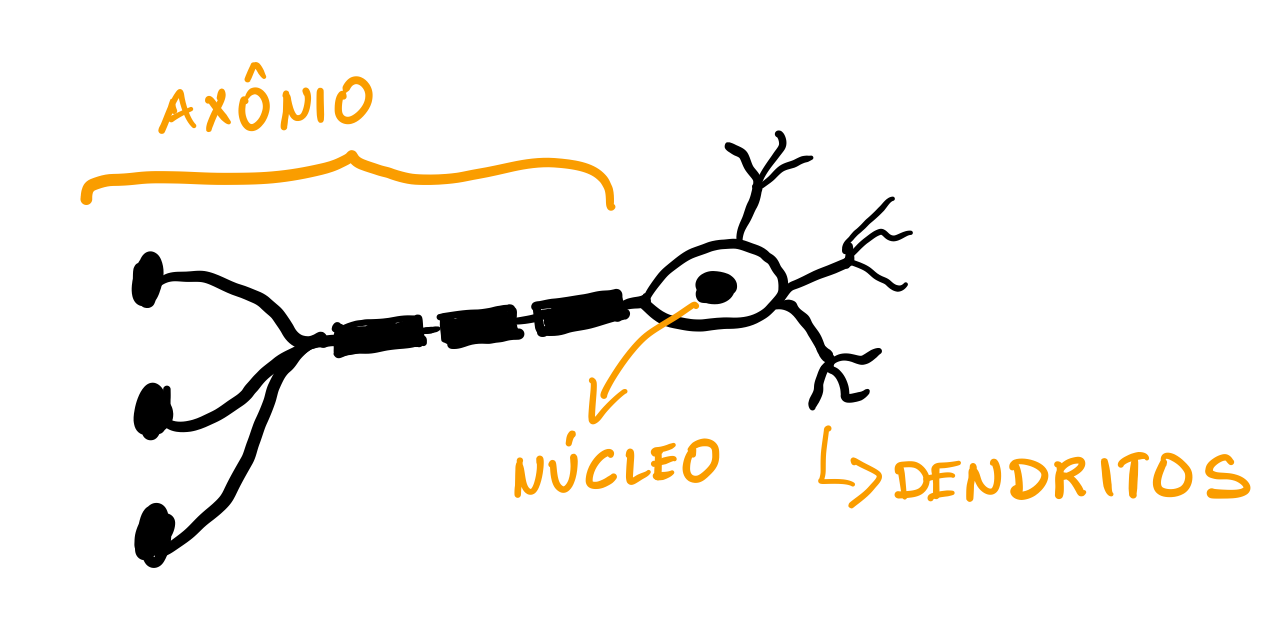
\includegraphics[scale=0.17]{./figs/Neural_Networks_Fig1.png}\hspace{1cm}
\end{center}
}

\Sli{
Matematicamente falando, podemos representar um neurônio da seguinte forma (Modelo de McCulloch-Pitts):

\begin{center}
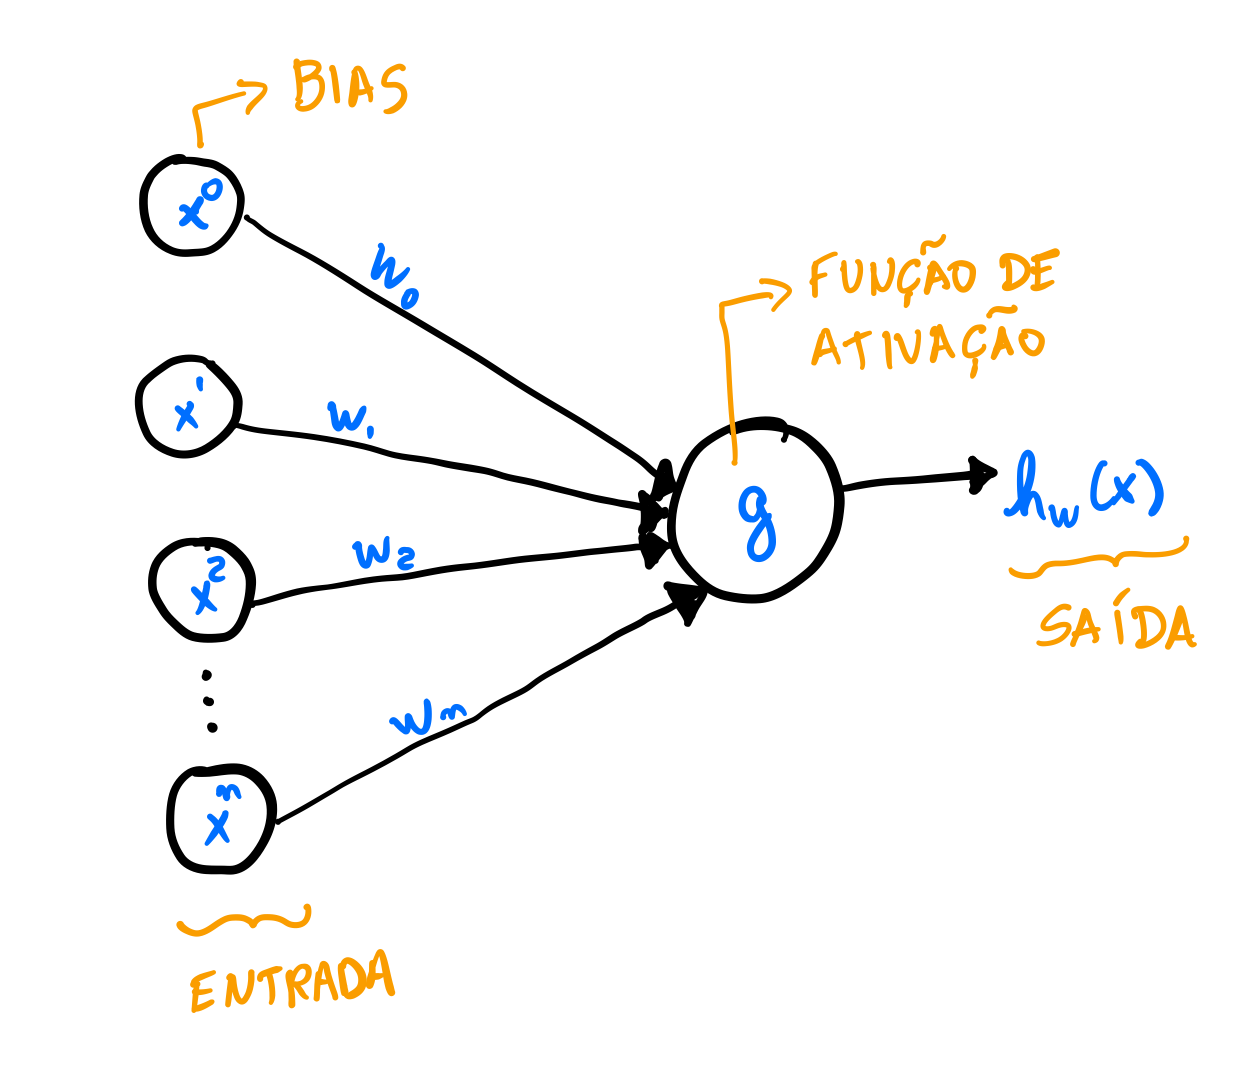
\includegraphics[scale=0.15]{./figs/Neural_Networks_Fig2.png}\hspace{1cm}
\end{center}
}

\Sli{
Alguns exemplos de funções de ativação:

\begin{itemize}
	\item Função logística (sigmoide): $g(a) = \frac{1}{1+e^{-a}}$, tal que $g(a)\in[0,1]$.
	\item Função limiar (degrau): 
	\begin{equation}\nonumber
		g_{\theta}(a) = 
		\begin{cases}
		1\text{ caso } \boldsymbol{w}^T\boldsymbol{x} \geq \theta\\
		0\text{ caso contrário}.
		\end{cases}
	\end{equation}
	tal que $g(a)\in\{0,1\}$.
	\item Função tangente hiperbólica: $g(a) = 2\sigma(2a)-1$, tal que $g(a)\in[-1,1]$ e $\sigma(x)$ corresponde à função logística.
\end{itemize}
}

\Sli{
É desejável que uma função de ativação seja \textbf{derivável}. Como escolhê-la? Depende de sua aplicação.

\begin{minipage}{0.49\textwidth}
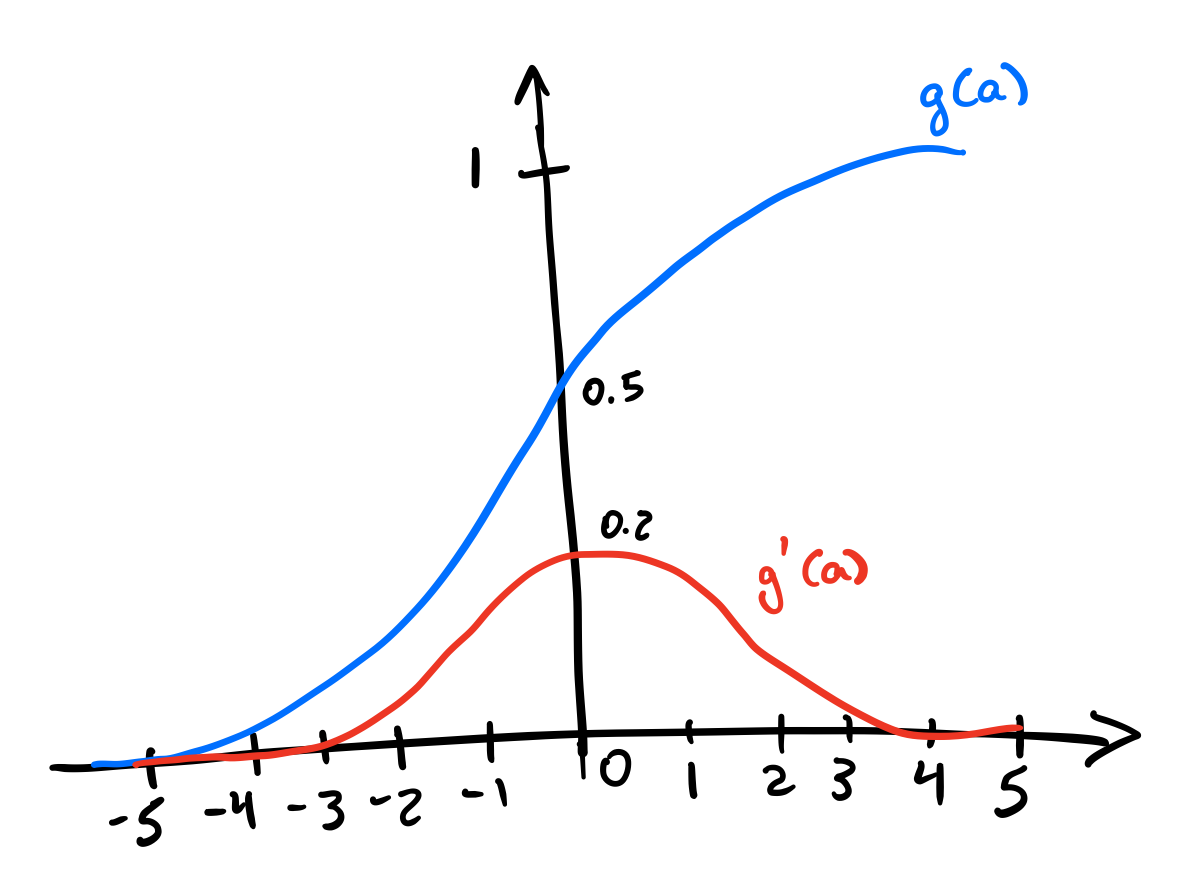
\includegraphics[scale=0.15]{./figs/Neural_Networks_Fig3.png}
\end{minipage}%%% to prevent a space
\begin{minipage}{0.37\textwidth}
Suponha $g(a) = \frac{1}{1+e^{-a}}$. Temos que $g^\prime(a) = g(a)(1-g(a))$. Note que $g^\prime(a)$ satura quando $a>5$ ou $a<-5$. Ademais, $g^\prime(a) <1$, $\forall a$. Isso significa que, para redes com muitas camadas, o gradiente tende a \textbf{desaparecer} durante o treinamento. 
\null
\par\xdef\tpd{\the\prevdepth}
\end{minipage}
}

\Sli{
\begin{minipage}{0.49\textwidth}
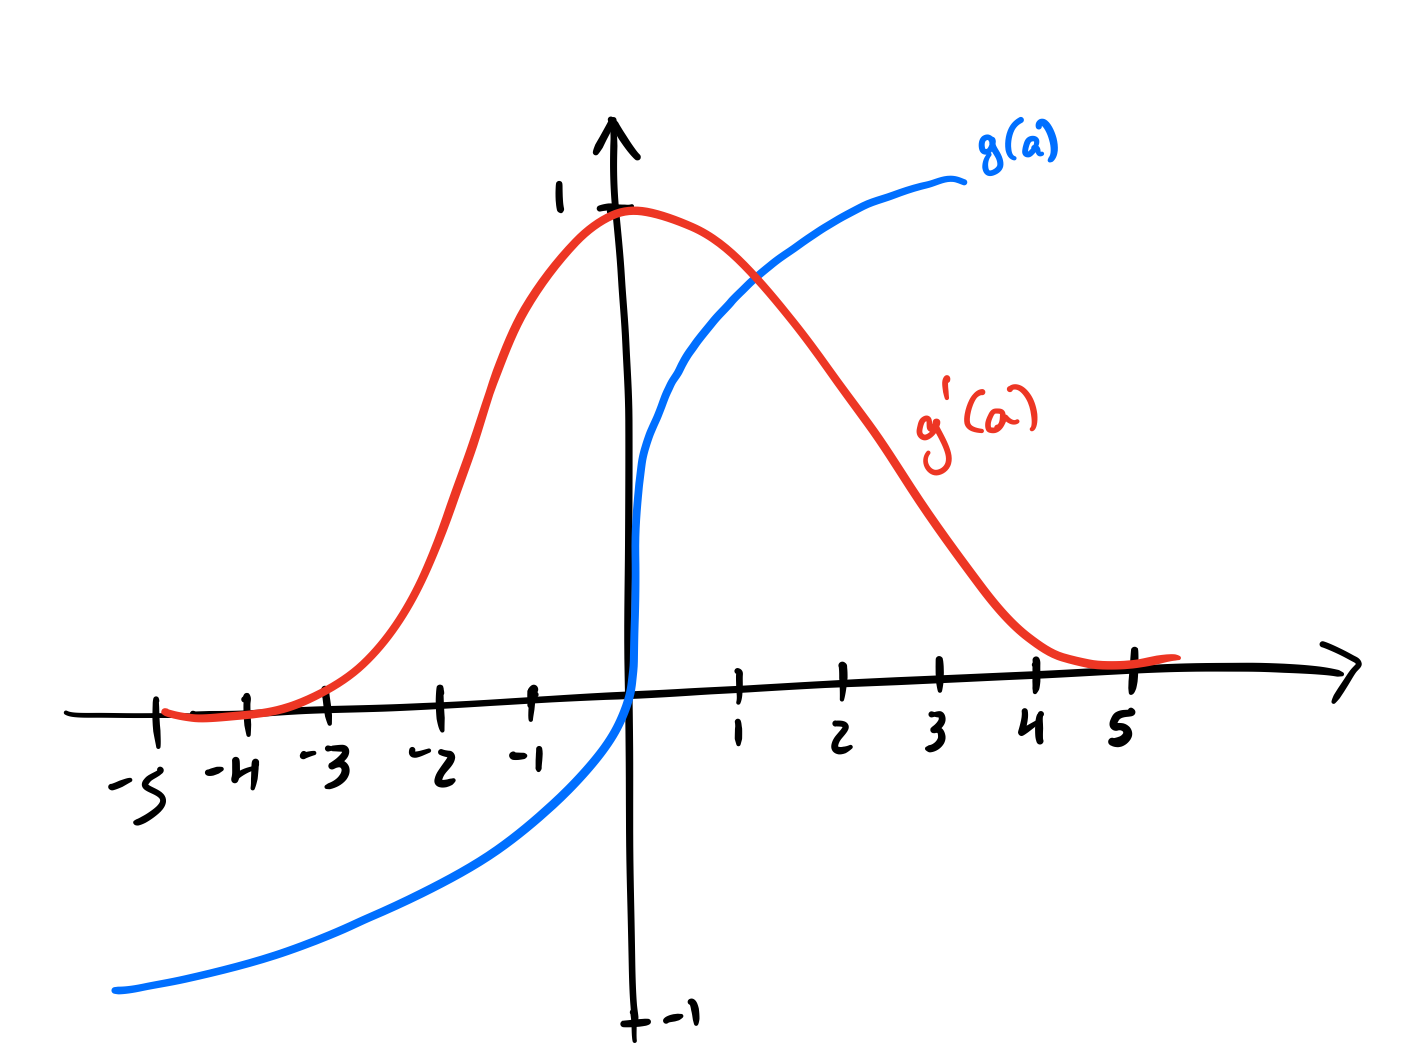
\includegraphics[scale=0.15]{./figs/Neural_Networks_Fig4.png}
\end{minipage}%%% to prevent a space
\begin{minipage}{0.37\textwidth}
Suponha $g(a) = 2\sigma(2a)-1$. Temos que $g^\prime(a) = 1-g^2(a)$. Muito embora saturações aconteçam, $g^\prime(a)$ atinge valores maiores, chegando, inclusive, ao máximo de $1$ quando $a=0$.
\null
\par\xdef\tpd{\the\prevdepth}
\end{minipage}
}

\Sli{
\secx{Perceptron}

\justify O Perceptron foi formalmente proposto por McCulloch e Pitts na década de 40 com o intuito de modelar matematicamente o neurônio humano. Muito embora ele tenha sido a base para muitos algoritmos, seu poder discriminativo é limitado, pois consegue aprender apenas hiperplanos como função de decisão.

\justify \underline{Definição do problema:} seja um conjunto de dados ${\cal X}= \{(\boldsymbol{x}_1,y_1),(\boldsymbol{x}_2,y_2),\ldots,(\boldsymbol{x}_z,y_z)\}$ tal que $\boldsymbol{x}_i\in\mathbb{R}^{n+1}$ corresponde ao dado de entrada e $y_i\in[-1,+1]$ denota o seu respectivo valor de saída. Temos, ainda, que ${\cal X}$ pode ser \textbf{particionado} da seguinte forma: ${\cal X} = {\cal X}^1\cup {\cal X}^2$, em que ${\cal X}^1$ e ${\cal X}^2$ denotam os conjuntos de dados de \textbf{treinamento} e \textbf{teste}, respectivamente. Nosso objetivo é, dado o conjunto de treinamento, aprender uma função $h:\mathbb{R}^{n+1}\rightarrow\{-1,+1\}$ que consiga atribuir a classe correta à uma determinada amostra.
}

\Sli{
\justify Vamos, agora, adaptar a função de ativação limiar para que possamos criar a nossa função hipótese:

\begin{equation}
	h_{\boldsymbol{w}}(\boldsymbol{x}) = 
	\begin{cases}
		+1\text{ caso }\boldsymbol{w}^T\boldsymbol{x}\geq \theta\\
		-1\text{ caso contrário.}
	\end{cases}
\end{equation}

\justify Para simplificar a notação, é usual trazermos $\theta$ para o lado esquerdo da equação e atribuirmos $w_0=\theta$. Novamente, consideraremos $x^0=1$. Assim, temos a função hipótese atualizada como segue:

\begin{equation}
	h_{\boldsymbol{w}}(\boldsymbol{x}) = 
	\begin{cases}
		+1\text{ caso }\boldsymbol{w}^T\boldsymbol{x}\geq 0\\
		-1\text{ caso contrário.}
	\end{cases}
\end{equation}
}

\Sli{
\justify Vamos, agora, revisitar alguns conceitos de Geometria Analítica. Suponha que tenhamos dois vetores $\boldsymbol{u} = [u_1\ u_2]$ e $\boldsymbol{v} = [v_1\ v_2]$. Geometricamente, podemos representá-los como segue:

\begin{minipage}{0.49\textwidth}
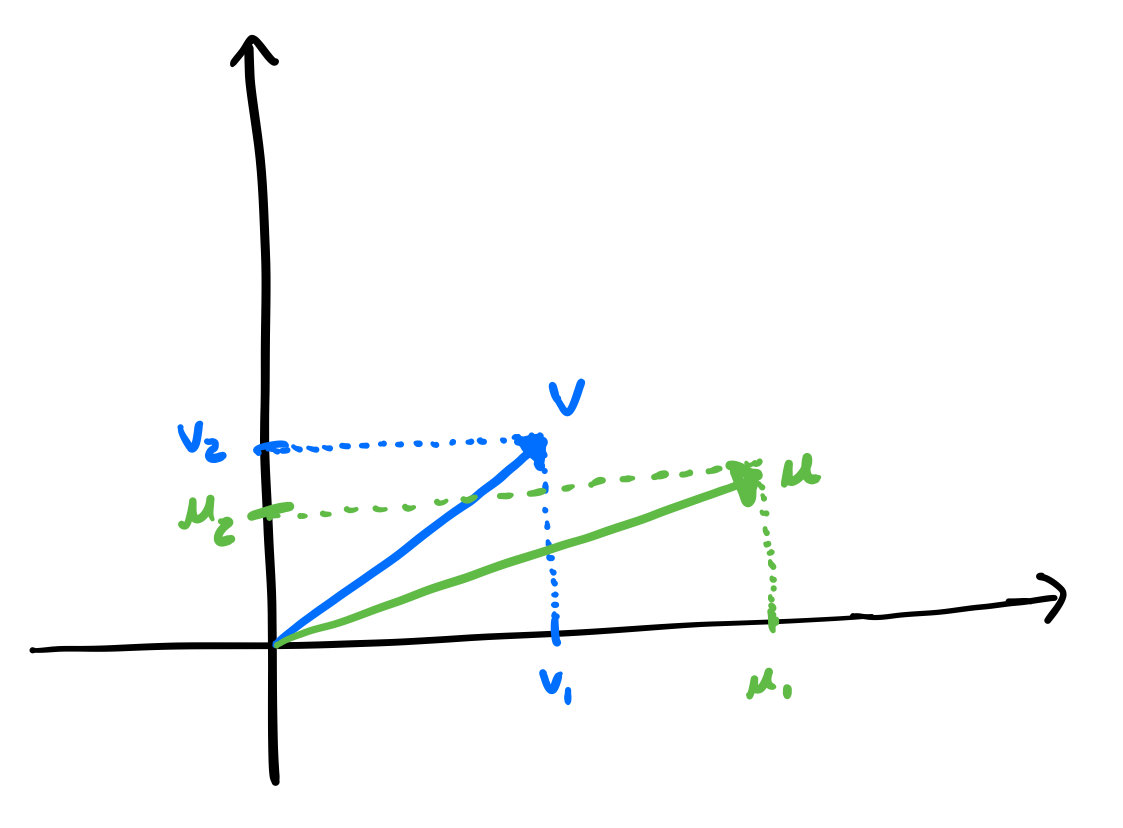
\includegraphics[scale=0.17]{./figs/Neural_Networks_Fig5.png}
\end{minipage}%%% to prevent a space
\begin{minipage}{0.37\textwidth}
Lembrando que $\norm{u} = \sqrt{u_1^2+u_2^2}$ denota o comprimento (magnitude) de $u$.
\null
\par\xdef\tpd{\the\prevdepth}
\end{minipage}
}

\Sli{
Temos, também, a definição de \textbf{projeção escalar} entre dois vetores, dada como segue:

\begin{minipage}{0.49\textwidth}
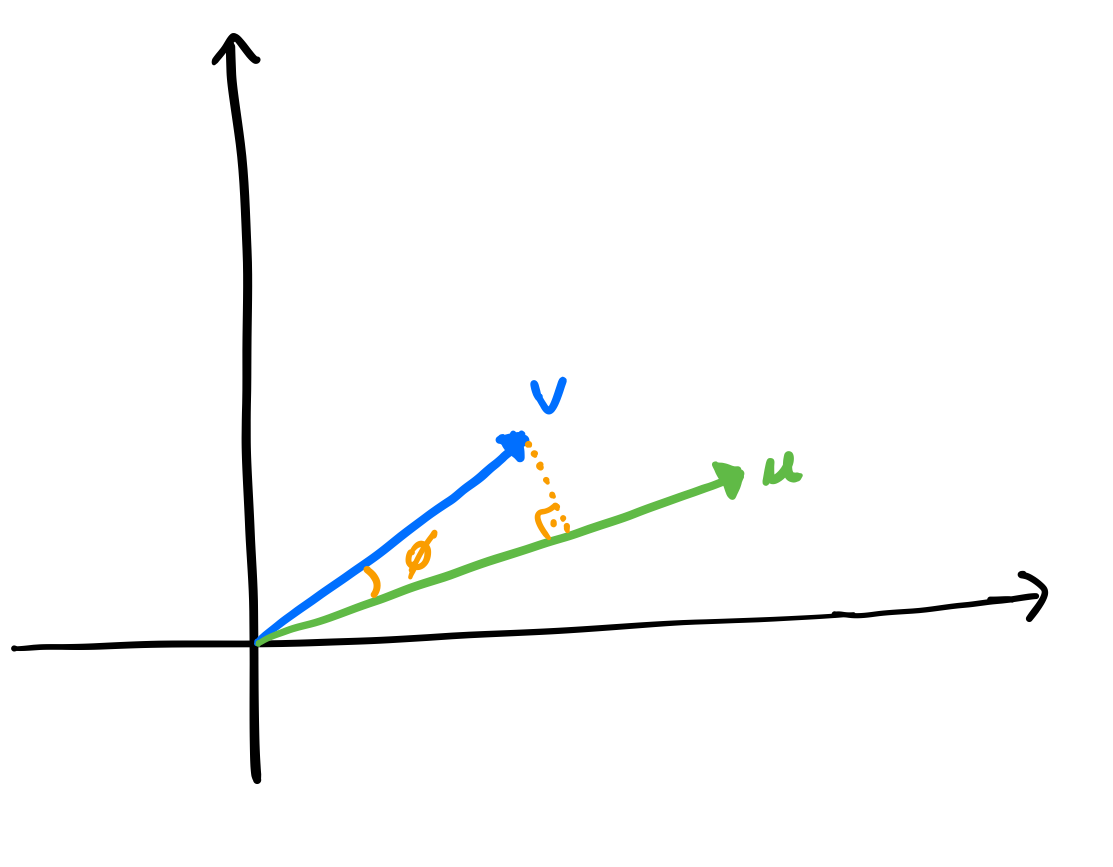
\includegraphics[scale=0.17]{./figs/Neural_Networks_Fig6.png}
\end{minipage}%%% to prevent a space
\begin{minipage}{0.43\textwidth}
Podemos, então, representar a projeção escalar entre dois vetores da seguinte forma: $\boldsymbol{w}^T\boldsymbol{x} = \norm{\boldsymbol{w}}.\cos\phi$. Lembrando que temos as seguintes situações:

	\begin{itemize}
		\item $\cos\phi > 0$ quando $0< \phi < 90\degree$.
		\item $\cos\phi < 0$ quando $90\degree < \phi < 270\degree$.
		\item $\cos\phi = 0$ quando $\phi = 90\degree$ ou $\phi = 270\degree$
	\end{itemize}
	
\null
\par\xdef\tpd{\the\prevdepth}
\end{minipage}
}

\Sli{
\justify Voltando ao nosso problema inicial, temos que a equação $\boldsymbol{w}^T\boldsymbol{x}=0$ define um hiperplano ortogonal ao vetor de pesos $\boldsymbol{w}$ deslocado de $-\theta$ (assumindo que $w_0=-\theta$ e $x_0 = 1$). Vamos supor 	que $\theta = 0$, ou seja, o hiperplano passa pela origem.

\begin{center}
	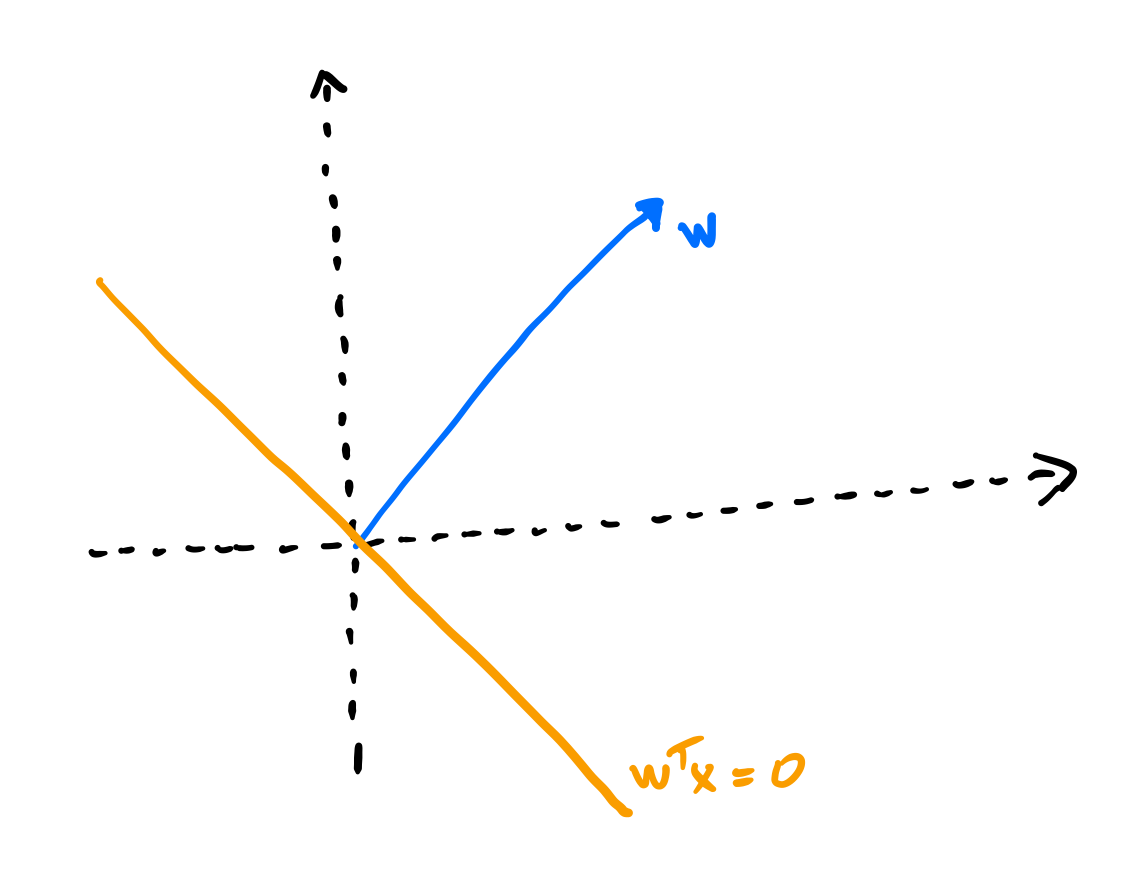
\includegraphics[scale=0.17]{./figs/Neural_Networks_Fig7.png}
\end{center}
}

\Sli{
\justify Como aprender o conjunto de pesos $\boldsymbol{w}$? A ideia intuitiva é \textbf{mover} o vetor de pesos de tal forma que as amostras fiquem posicionadas corretamente no espaço de características. No exemplo abaixo, temos um conjunto de dados ${\cal X}^1=\{(\boldsymbol{x}_1,+1),(\boldsymbol{x}_2,+1),(\boldsymbol{x}_3,-1),(\boldsymbol{x}_4,-1)\}$, de tal forma que o hiperplano $\boldsymbol{w}^T\boldsymbol{x}=0$ já se encontra posicionado corretamente.

\begin{minipage}{0.49\textwidth}
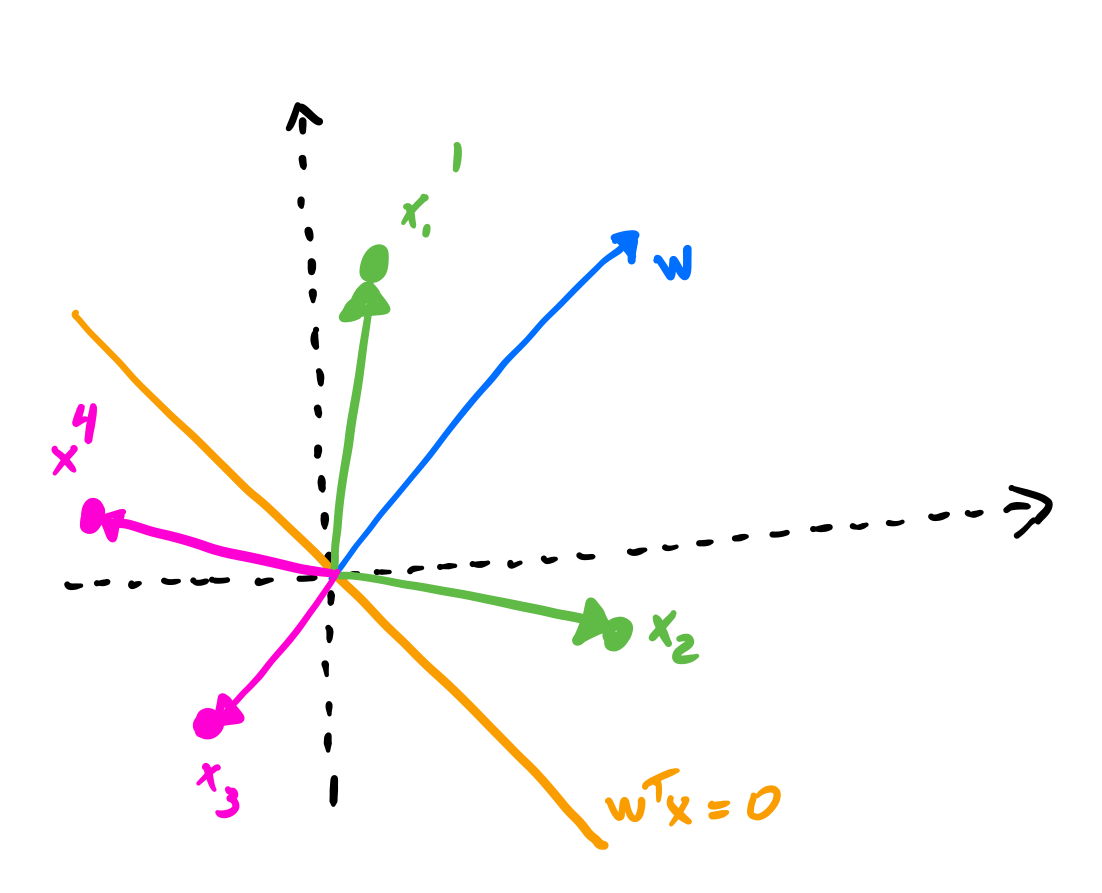
\includegraphics[scale=0.17]{./figs/Neural_Networks_Fig8.png}
\end{minipage}%%% to prevent a space
\begin{minipage}{0.5\textwidth}
A regra de atualização dos pesos é dada pela seguinte fórmula:

\begin{equation}
	\boldsymbol{w}^{(t+1)} = \boldsymbol{w}^{(t)}+\alpha(y_i-h_{\boldsymbol{w}^{(t)}}(\boldsymbol{x}_i))\boldsymbol{x}_i,
\end{equation}
tal que $\forall i = 1,2,\ldots,m$. 
\null
\par\xdef\tpd{\the\prevdepth}
\end{minipage}

}

\Sli{
\justify Mas como ele funciona na prática? Suponha uma amostra $\boldsymbol{x}\in{\cal X}$ tal que $y = +1$ e $h_{\boldsymbol{w}}(\boldsymbol{x})=-1$. Para um valor de $\alpha = 0.5$, tempos que:

\begin{align}\nonumber
	\boldsymbol{w}^{(t+1)} &= \boldsymbol{w}^{(t)}+\alpha(1-(-1))\boldsymbol{x}\\
	&=\boldsymbol{w}^{(t)}+0.5(2)\boldsymbol{x} = \boldsymbol{w}^{(t)}+\boldsymbol{x}.
\end{align}
Desta forma, o vetor de pesos $\boldsymbol{w}$ será rotacionado de modo que $\boldsymbol{x}$ seja positivo.
\vspace{-0.5cm}
\begin{center}
\begin{tabular}{ccc}
	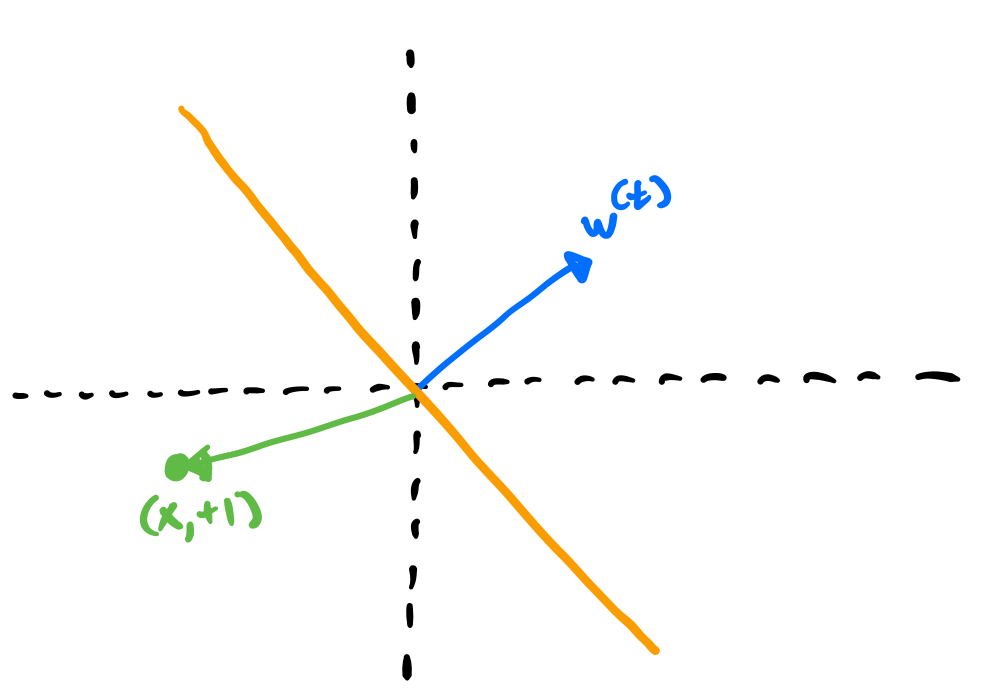
\includegraphics[scale=0.127]{./figs/Neural_Networks_Fig9.png} &
	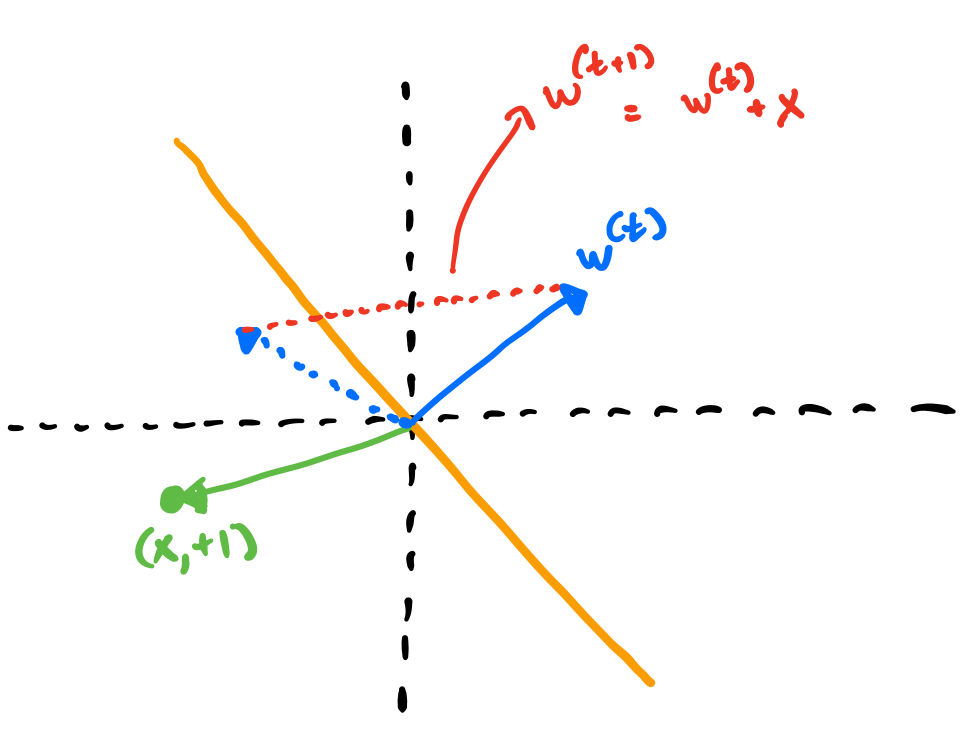
\includegraphics[scale=0.127]{./figs/Neural_Networks_Fig10.png} &
	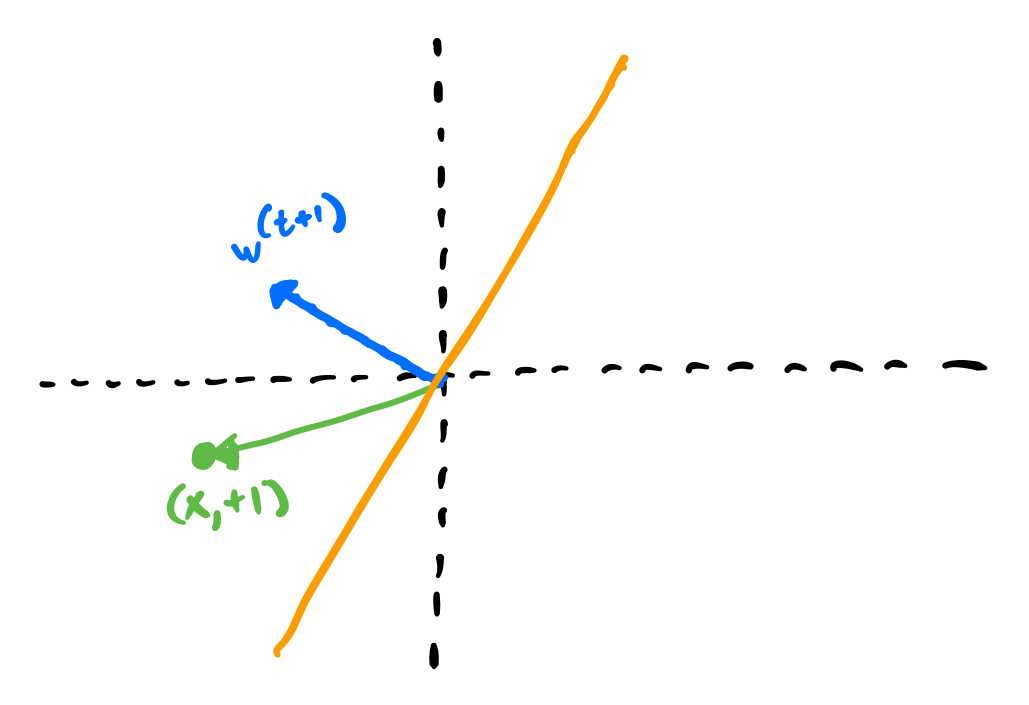
\includegraphics[scale=0.127]{./figs/Neural_Networks_Fig11.png} \\
	Predição & Atualização & Hiperplano aprendido
\end{tabular}
\end{center}
}

\Sli{
\justify De maneira análoga, caso o rótulo de $\boldsymbol{x}$ seja negativo, ou seja, $y=-1$, temos que:

\begin{align}\nonumber
	\boldsymbol{w}^{(t+1)} &= \boldsymbol{w}^{(t)}+\alpha(-1-(+1))\boldsymbol{x}\\
	&=\boldsymbol{w}^{(t)}+0.5(-2)\boldsymbol{x} = \boldsymbol{w}^{(t)}-\boldsymbol{x}.
\end{align}
\justify Assim, o vetor de pesos será rotacionado (por meio das projeções) para o outro lado. Para um conjunto de dados que seja \textbf{linearmente separável}, foi provado matematicamente que o algoritmo do Perceptron tem sua \textbf{convergência garantida}.
}

\Sli{
Como funciona o seu algoritmo? Vamos lá:

\begin{enumerate}
	\item Atribua pesos aleatórios para $\boldsymbol{w}$.
	\item Inicialize $\alpha$.
	\item $t=0$.
	\item Para cada amostra $\boldsymbol{x}_i\in{\cal X}^1$, faça:
	\begin{enumerate} 
	\item $\boldsymbol{w}^{(t+1)} = \boldsymbol{w}^{(t)}+\alpha(y_i-h_{\boldsymbol{w}^{(t)}}(\boldsymbol{x}_i))\boldsymbol{x}_i$
	\end{enumerate}
	\item Repita o passo 4 até algum critério de convergência for estabelecido.	
\end{enumerate}
}

\Sli{
\justify Vejamos alguns exemplos de funcionamento do Perceptron. Considere o problema de resolver a seguinte equação lógica: $y = x^1$ AND $x^2$. Para duas entradas, temos $2^2$ possibilidades de amostras, isto é, o nosso conjunto de dados é composto pelos seguintes elementos: ${\cal X}=\{([0\ 0],0),([0\ 1],0),([1\ 0],0),([1\ 1],1)\}$. Conseguimos encontrar o hiperplano separador?

\begin{minipage}{0.32\textwidth}
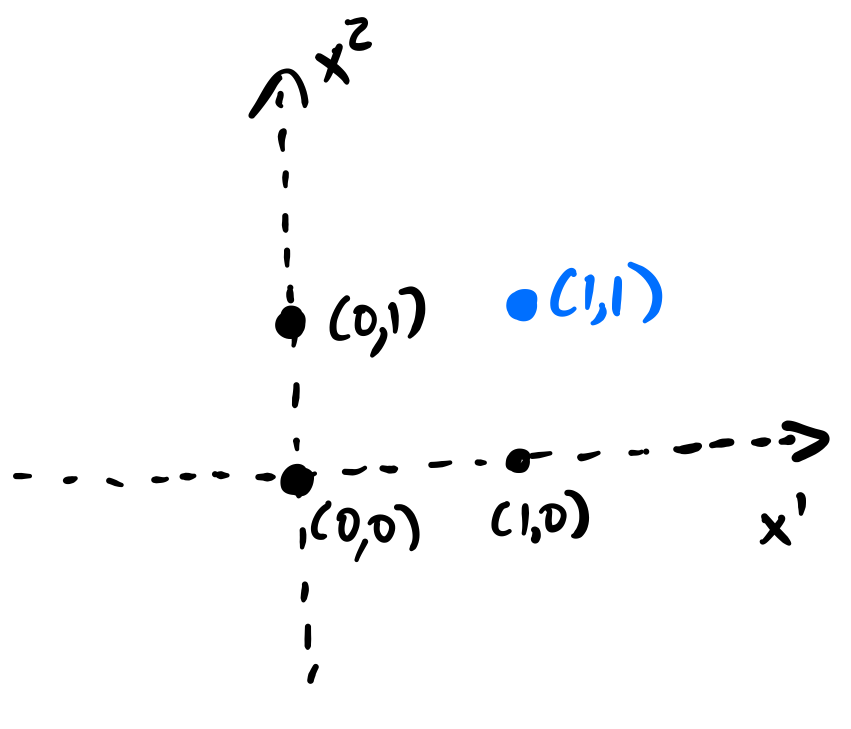
\includegraphics[scale=0.15]{./figs/Neural_Networks_Fig12.png}
\end{minipage}%%% to prevent a space
\begin{minipage}{0.32\textwidth}
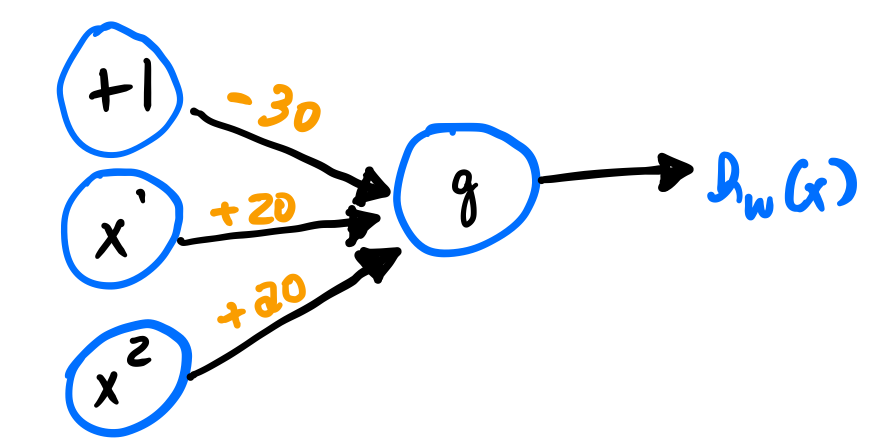
\includegraphics[scale=0.15]{./figs/Neural_Networks_Fig13.png}
\end{minipage}%%% to prevent a space
\begin{minipage}{0.32\textwidth}
\scriptsize
Nossa função hipótese é dada por $h_{\boldsymbol{w}}(\boldsymbol{x})=g(-30+20x^1+20x^2)$. Utilizando $g$ como uma função logística, temos que:
\begin{table}[]
\begin{tabular}{lll}
\rowcolor[HTML]{EFEFEF} 
$x^1$ & $x^2$ & $h_{\boldsymbol{w}}(\boldsymbol{x})$                      \\
0  & 0  & $g(-30)\approx 0$ \\
0  & 1  & $g(-10)\approx 0$ \\
1  & 0  & $g(-10)\approx 0$ \\
1  & 1  & $g(10)\approx 1$ \\
\end{tabular}
\end{table}
\null
\par\xdef\tpd{\the\prevdepth}
\end{minipage}
}

\Sli{
\justify Considere, agora, o problema de resolver a seguinte equação lógica: $y = x^1$ OR $x^2$. Para duas entradas, temos $2^2$ possibilidades de amostras, isto é, o nosso conjunto de dados é composto pelos seguintes elementos: ${\cal X}=\{([0\ 0],0),([0\ 1],1),([1\ 0],1),([1\ 1],1)\}$. Conseguimos encontrar o hiperplano separador?

\begin{minipage}{0.32\textwidth}
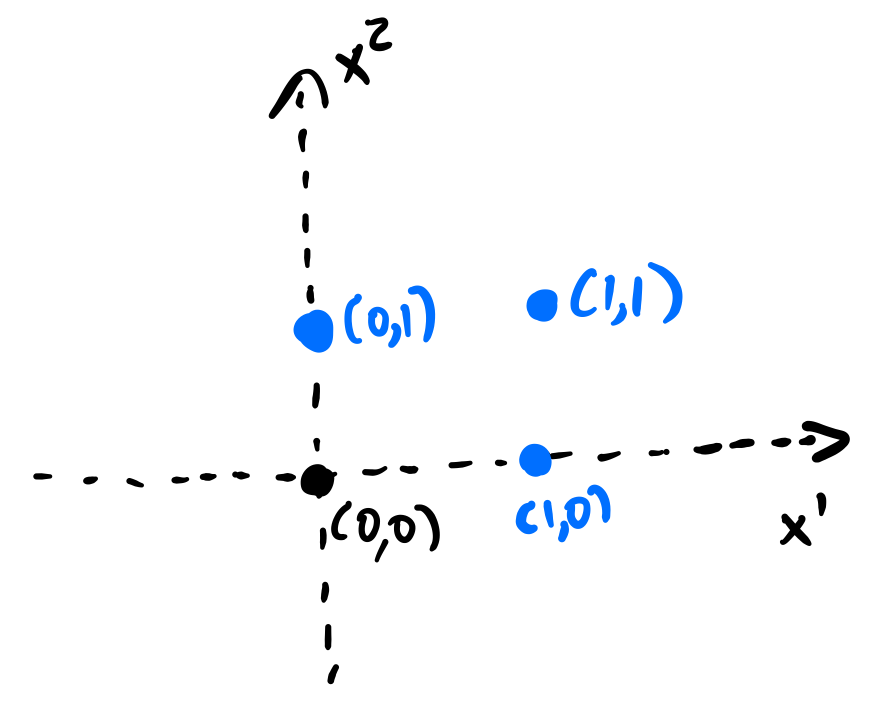
\includegraphics[scale=0.15]{./figs/Neural_Networks_Fig14.png}
\end{minipage}%%% to prevent a space
\begin{minipage}{0.32\textwidth}
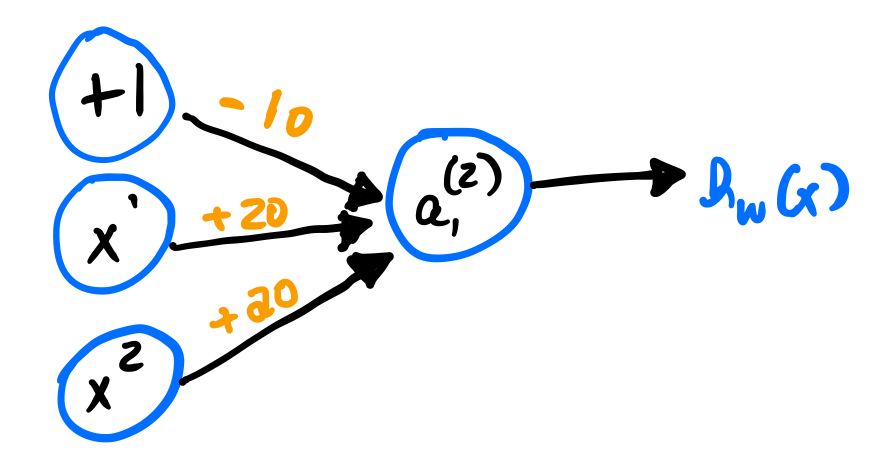
\includegraphics[scale=0.15]{./figs/Neural_Networks_Fig15.png}
\end{minipage}%%% to prevent a space
\begin{minipage}{0.32\textwidth}
\scriptsize
Nossa função hipótese é dada por $h_{\boldsymbol{w}}(\boldsymbol{x})=g(-10+20x^1+20x^2)$. Utilizando $g$ como uma função logística, temos que:
\begin{table}[]
\begin{tabular}{lll}
\rowcolor[HTML]{EFEFEF} 
$x^1$ & $x^2$ & $h_{\boldsymbol{w}}(\boldsymbol{x})$                      \\
0  & 0  & $g(-10)\approx 0$ \\
0  & 1  & $g(10)\approx 1$ \\
1  & 0  & $g(10)\approx 1$ \\
1  & 1  & $g(30)\approx 1$ \\
\end{tabular}
\end{table}
\null
\par\xdef\tpd{\the\prevdepth}
\end{minipage}
}

\Sli{
\justify Considere, agora, o problema de resolver a seguinte equação lógica: $y = $ NOT $x^1$. Agora temos apenas uma entrada, ou seja, $x^1$. Assim, o nosso conjunto de dados é composto pelos seguintes elementos: ${\cal X}=\{(0,1),(1,0)\}$. Conseguimos encontrar o hiperplano separador?

\begin{center}
\begin{minipage}{0.4\textwidth}
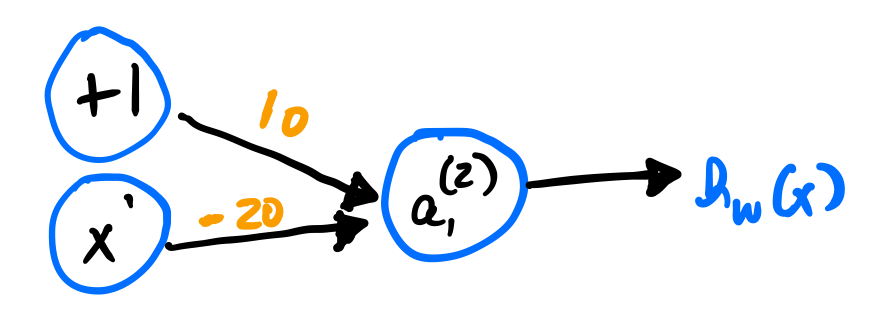
\includegraphics[scale=0.15]{./figs/Neural_Networks_Fig16.png}
\end{minipage}%%% to prevent a space
\begin{minipage}{0.32\textwidth}
\scriptsize
Nossa função hipótese é dada por $h_{\boldsymbol{w}}(\boldsymbol{x})=g(10-20x^1)$. Utilizando $g$ como uma função logística, temos que:
\begin{table}[]
\begin{tabular}{ll}
\rowcolor[HTML]{EFEFEF} 
$x^1$ & $h_{\boldsymbol{w}}(\boldsymbol{x})$                      \\
0  & $g(10)\approx 1$ \\
1  & $g(-10)\approx 0$ \\
\end{tabular}
\end{table}
\null
\par\xdef\tpd{\the\prevdepth}
\end{minipage}
\end{center}
}

\Sli{
\justify O que seria então uma Rede Neural do tipo Perceptron Multicamadas (\emph{Multilayer Perceptron} - MLP)? Basicamente, é um grupo de neurônios que, combinados, permitem o aprendizado de um número maior de funções de decisão.

\begin{center}
	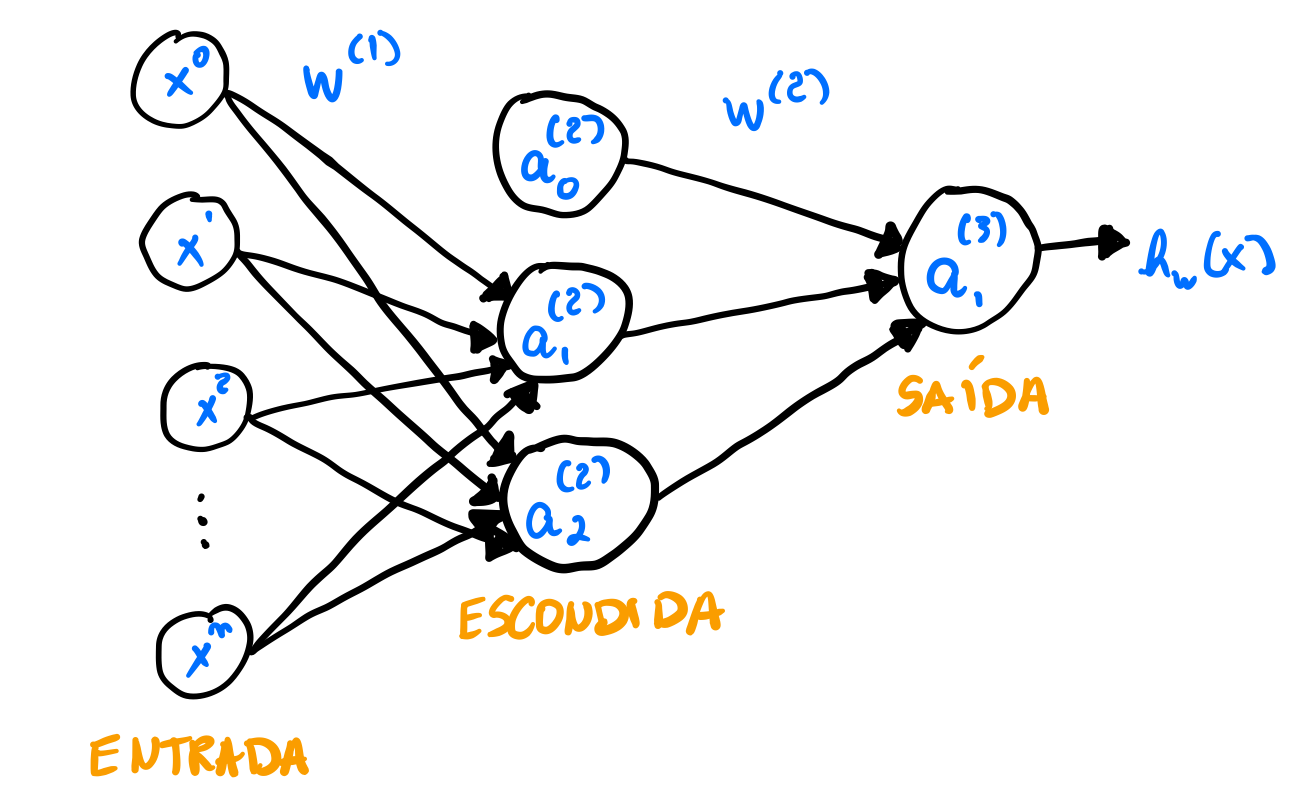
\includegraphics[scale=0.13]{./figs/Neural_Networks_Fig17.png}
\end{center}

Na ilustração acima, temos que $a^{(j)}_i$ denota o neurônio $i$ da camada $j$, e $\boldsymbol{W}^{(l)}$ é a matriz de pesos que conecta as camadas $l$ e $l+1$. Essa arquitetura é geralmente representada por $n$:$3$:$1$.
}

\Sli{
Considerando a rede neural anterior, vamos analisar uma situação mais específica.

\begin{center}
\begin{minipage}{0.33\textwidth}
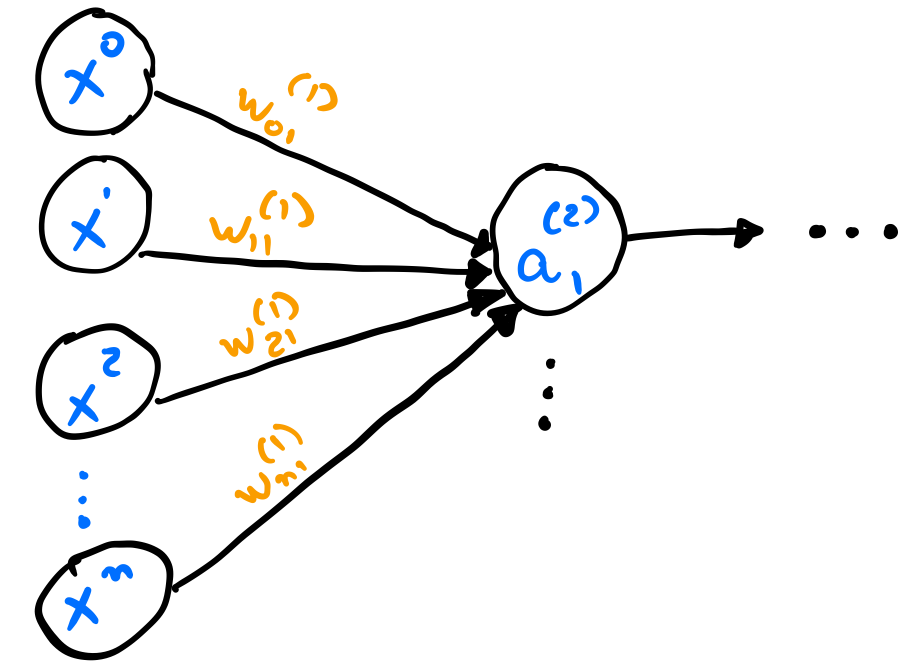
\includegraphics[scale=0.13]{./figs/Neural_Networks_Fig18.png}
\end{minipage}%%% to prevent a space
\begin{minipage}{0.47\textwidth}
\scriptsize
\begin{align}\nonumber
a^{(2)}_1 &= g(\underbrace{w^{(1)}_{01}x^0+w^{(1)}_{11}x^1+w^{(1)}_{02}x^2+\ldots+w^{(1)}_{0n}x^n}_{\displaystyle \sum_{i=0}^n w^{(1)}_{i1}x^i=b^{(2)}_1})
\end{align}
\null
\par\xdef\tpd{\the\prevdepth}
\end{minipage}
\end{center}
A função de decisão final da rede neural é dada pela seguinte formulação:

\begin{equation}
	h_{\boldsymbol{x}}(\boldsymbol{w}) = a^{(3)}_1 = g\left(w^{(2)}_{01}a^{(2)}_0+w^{(2)}_{11}a^{(2)}_1+w^{(2)}_{21}a^{(2)}_2\right).
\end{equation}
}

\Sli{
\justify E no caso de problemas com múltiplas classes? Neste caso, para um problema com $c$ classes, nossa camada de saída necessita de $c$ neurônios.

\begin{center}
\begin{minipage}{0.33\textwidth}
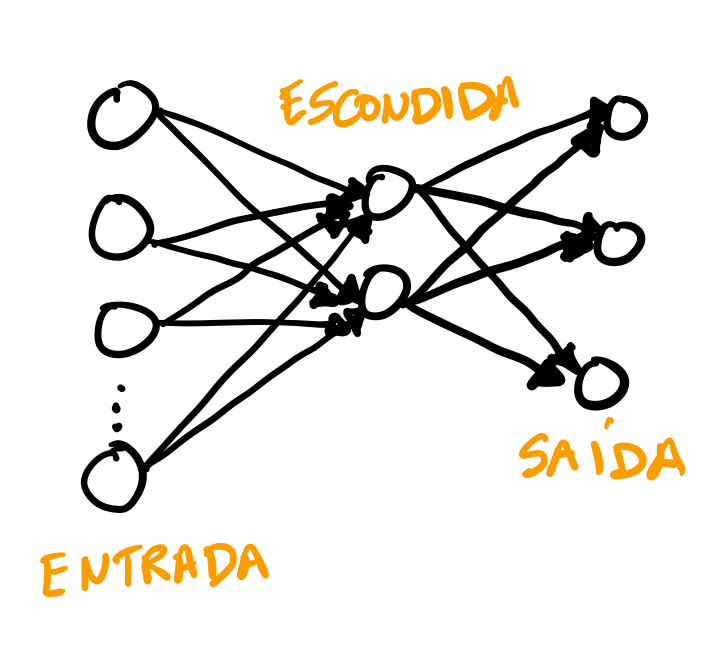
\includegraphics[scale=0.17]{./figs/Neural_Networks_Fig19.png}
\end{minipage}%%% to prevent a space
\begin{minipage}{0.47\textwidth}
Podemos utilizar a metodologia de codificação \emph{one-hot} para representar cada neurônio de saída, em que $\boldsymbol{h}_{\boldsymbol{w}}(\boldsymbol{x})\in\mathbb{R}^3$:\\\\
\begin{tabular}{ccc}
$h^1_{\boldsymbol{w}}(\boldsymbol{x}) \approx 
\begin{bmatrix}
1 \\
0 \\
0
\end{bmatrix}
$ &
$h^2_{\boldsymbol{w}}(\boldsymbol{x}) \approx 
\begin{bmatrix}
0 \\
1 \\
0
\end{bmatrix}
$ &
$h^3_{\boldsymbol{w}}(\boldsymbol{x}) \approx 
\begin{bmatrix}
0 \\
0 \\
1
\end{bmatrix}
$\\
Classe 1 & Classe 2 & Classe 3	
\end{tabular}
\null
\par\xdef\tpd{\the\prevdepth}
\end{minipage}
\end{center}
O mesmo acontece com o rótulo $y$ de cada amostra, que passa a ser agora um vetor $\boldsymbol{y}\in\mathbb{R}^3$.
}

\Sli{
\justify Existem diversos algoritmos de treinamento para Redes Neurais MLP, em que o mais conhecido é chamado de \textbf{retropropagação}, do inglês \emph{backpropagation}. Ele possui dois passos: (i) propagação para frente (\emph{forward propagation}) e (ii) propagação para trás (\emph{backpropagation}). Antes de estudarmos o seu funcionamento, vamos dar uma olhada na função de custo:

\begin{equation}
	J(\boldsymbol{w}) = \frac{1}{m}\left[\sum_{i=1}^m\sum_{k=1}^c-y_i^k\log(h^k_{\boldsymbol{w}}(\boldsymbol{x}_i))-(1-y_i^k)\log(1-h^k_{\boldsymbol{w}}(\boldsymbol{x}_i))\right].
\end{equation}
Fazendo uma analogia, a formulação acima contempla uma rede neural com $c$ regressores logísticos caso tenhamos uma função de ativação logística na camada de saída.
}

\Sli{
\justify Podemos utilizar, novamente, o gradiente descendente para otimizar a função de custo $J(\boldsymbol{w})$. No entanto, note que o problema passa a ser mais complexo, pois precisamos calcular as derivadas parciais com relação à todos os pesos da rede, ou seja:

\begin{equation}
\frac{\partial J(\boldsymbol{w})}{\partial w^{(l)}_{ij}},
\end{equation}
em que $l=1,2,\ldots,L-1$ tal que $L$ denota a quantidade de camadas da rede neural.
}

\Sli{
\justify Seja uma rede do tipo $3$:$4$:$4$:$2$ ilustrada abaixo. Suponha que tenhamos apenas uma amostra no conjunto de treinamento. Neste caso, o passo \emph{forward} é dado pelas seguintes etapas:

\begin{minipage}{0.57\textwidth}
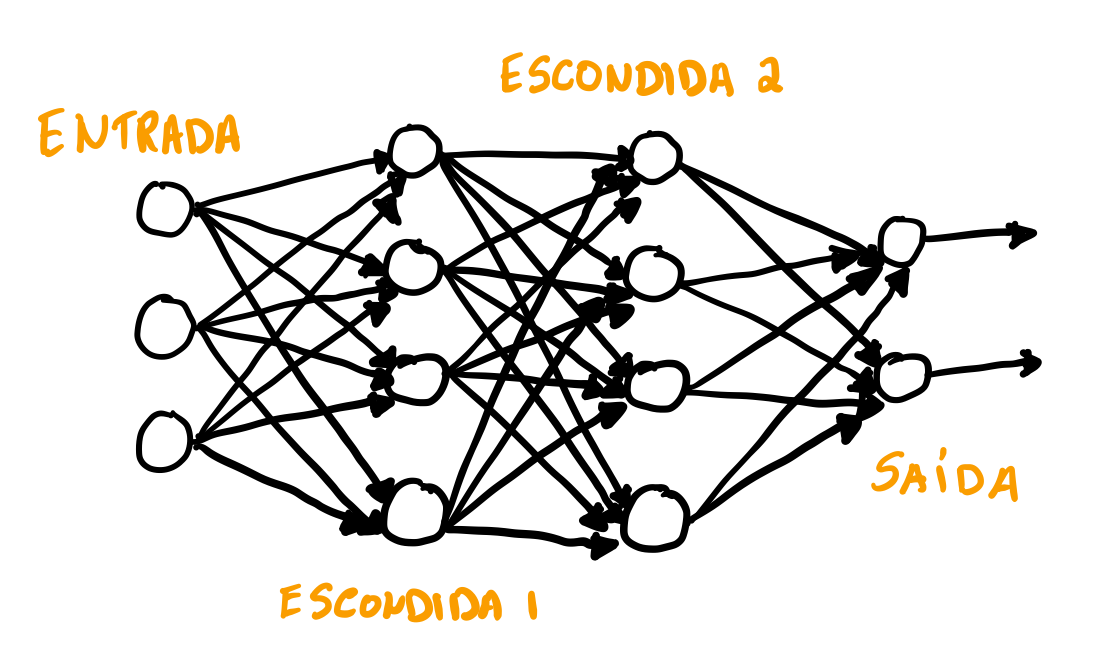
\includegraphics[scale=0.2]{./figs/Neural_Networks_Fig20.png}
\end{minipage}%%% to prevent a space
\begin{minipage}{0.47\textwidth}
\begin{enumerate}
	\item $\boldsymbol{a}^{(1)}\leftarrow\boldsymbol{x}$
	\item $\boldsymbol{b}^{(2)}\leftarrow\left(\boldsymbol{W}^{(1)}\right)^T\boldsymbol{a}^{(1)}$
	\item $\boldsymbol{a}^{(2)}\leftarrow g\left(\boldsymbol{b}^{(2)}\right)$
	\item $\boldsymbol{b}^{(3)}\leftarrow\left(\boldsymbol{W}^{(2)}\right)^T\boldsymbol{a}^{(2)}$
	\item $\boldsymbol{a}^{(3)}\leftarrow g\left(\boldsymbol{b}^{(3)}\right)$
	\item $\boldsymbol{b}^{(4)}\leftarrow\left(\boldsymbol{W}^{(3)}\right)^T\boldsymbol{a}^{(3)}$
	\item $h_{\boldsymbol{w}}(\boldsymbol{x}) = \boldsymbol{a}^{(4)}\leftarrow g\left(\boldsymbol{b}^{(4)}\right)$
\end{enumerate}
\null
\par\xdef\tpd{\the\prevdepth}
\end{minipage}
}

\Sli{
\justify Para o passo de \emph{backpropagation}, temos a definição de uma nova variável $\delta^{(l)}_{j}$ que denota um erro parcial acumulado no neurônio $j$ da camada $l$. Este erro deve ser calculado de forma diferente para os neurônios de saída e das camada escondidas, como segue:

\begin{itemize}
	\item Camada de saída ($l=4$):
	\begin{align}\nonumber
	\delta^{(4)}_j &= a^{(4)}_j-y^j\\ &=h^j_{\boldsymbol{w}}(\boldsymbol{x})-y^j
	\end{align}
	Em notação vetorial, temos que $\boldsymbol{\delta}^{(4)} = \boldsymbol{a}^{(4)}-\boldsymbol{y} = \boldsymbol{h}_{\boldsymbol{w}}(\boldsymbol{x})-\boldsymbol{y}$.
\end{itemize}
}

\Sli{
\begin{itemize}
	\item Camadas escondidas $l=\{2,3\}$:
	\begin{itemize}
	\item $\boldsymbol{\delta}^{(3)} = \left(\boldsymbol{W}^{(3)}\right)^T\boldsymbol{\delta}^{(4)}.*g^\prime\left(\boldsymbol{b}^{(3)}\right)$
	\item $\boldsymbol{\delta}^{(2)} = \left(\boldsymbol{W}^{(2)}\right)^T\boldsymbol{\delta}^{(3)}.*g^\prime\left(\boldsymbol{b}^{(2)}\right)$
	\end{itemize}
Na prática, temos a seguinte formulação para propagação dos erros nas camadas intermediárias:
\end{itemize}

\begin{equation}
	\boldsymbol{\delta}^{(l)} = \left(\boldsymbol{W}^{(l)}\right)^T\boldsymbol{\delta}^{(l+1)}.*g^\prime\left(\boldsymbol{b}^{(l)}\right).
\end{equation}		
}

\Sli{
O nome \textbf{retropropagação} deve-se ao fato de o algoritmo ``propagar para trás"\ o erro estimado em cada camada. As derivadas parciais podem ser calculadas como segue:

\begin{equation}
	\frac{\partial J(\boldsymbol{w})}{\partial w^{(l)}_{ij}} = a^{(l)}_i\delta^{(l+1)}_j.
\end{equation}
Note, então, que as derivadas parciais são calculadas com relação à todos os pesos da rede neural.
}

\Sli{
Segue algoritmo de retropropagação para treinamento de uma rede neural MLP.

\begin{enumerate}
	\item Atribua pesos aleatórios para $w^{(l)}_{ij}$\ \ $\forall l,i,j$
	\item Execute os passos abaixo ate o critério de parada ter sido estabelecido: \textcolor{gray}{\ \ Laço das épocas}
	\begin{enumerate}
		\item $\Delta^{(l)}_{ij} = 0$\ \ $\forall l,i,j$ \textcolor{gray}{\ \ \ Variável utilizada para armazenar $\frac{\partial J(\boldsymbol{w})}{\partial w^{(l)}_{ij}}$}
		\item Para cada amostra $\boldsymbol{x}_i\in{\cal X}^1$, faça:
		\begin{enumerate}
		\item Execute o passo de \emph{forward propagation} para calcular $\boldsymbol{a}^{l}$,\ \ $l = 2,3,\ldots,L$
		\item Execute o passo de \emph{backward propagation} para calcular:
			\begin{itemize}
				\item $\boldsymbol{\delta}^{l}$,\ \ $l = L,L-1,\ldots,2$\textcolor{gray}{\ \ \ Erro em cada neurônio}
				\item $\Delta^{(l)}_{ij} = \Delta^{(l)}_{ij}+a^{(l)}_i\delta^{(l+1)}_j$\textcolor{gray}{\ \ \ Derivadas parciais são acumuladas}
			\end{itemize}
		\end{enumerate}
		\item $D^{(l)}_{ij} = \frac{1}{m}\Delta^{(l)}_{ij}$\ \ $\forall l,i,j$ \textcolor{gray}{\ \ \ Calcula o gradiente médio}
		\item $w^{(l)}_{ij} = w^{(l)}_{ij}-\alpha D^{(l)}_{ij}$\ \ $\forall l,i,j$ \textcolor{gray}{\ \ \ Atualiza pesos com gradiente descendente}
		\item Avalie a função de custo $J(\boldsymbol{w})$
	\end{enumerate}
\end{enumerate}
}

\Sli{
Resumindo: passo \emph{forward}.

\begin{center}
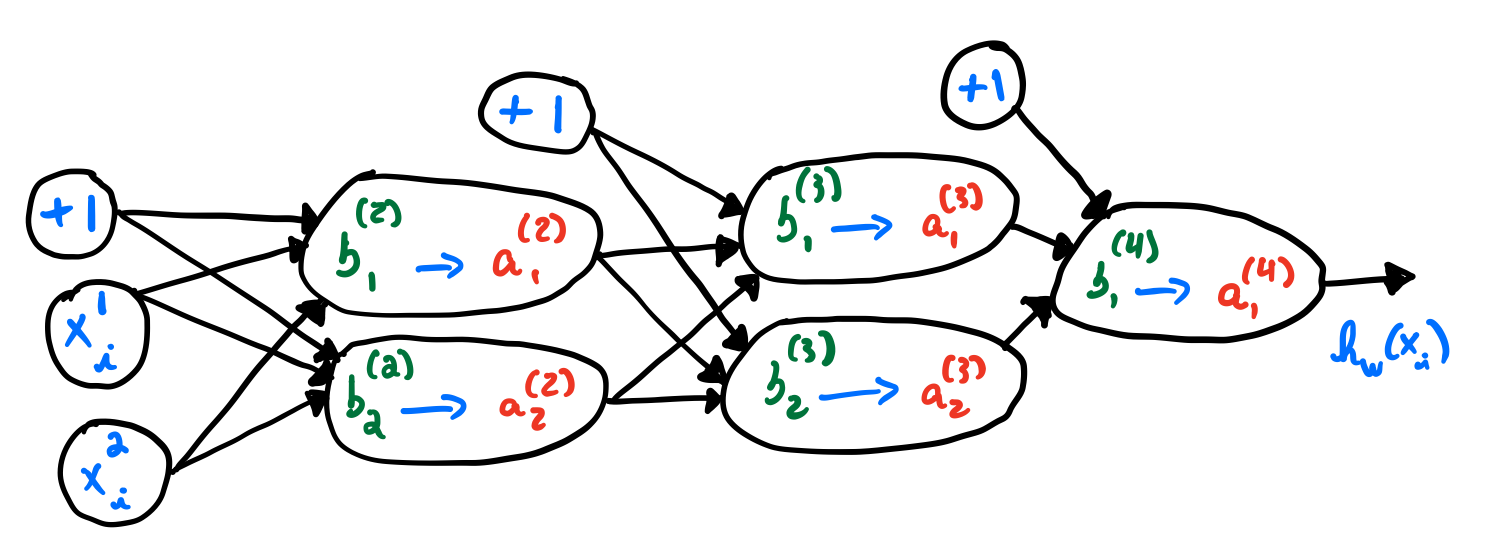
\includegraphics[scale=0.2]{./figs/Neural_Networks_Fig21.png}
\end{center}
}

\Sli{
Resumindo: passo \emph{backward}.

\begin{center}
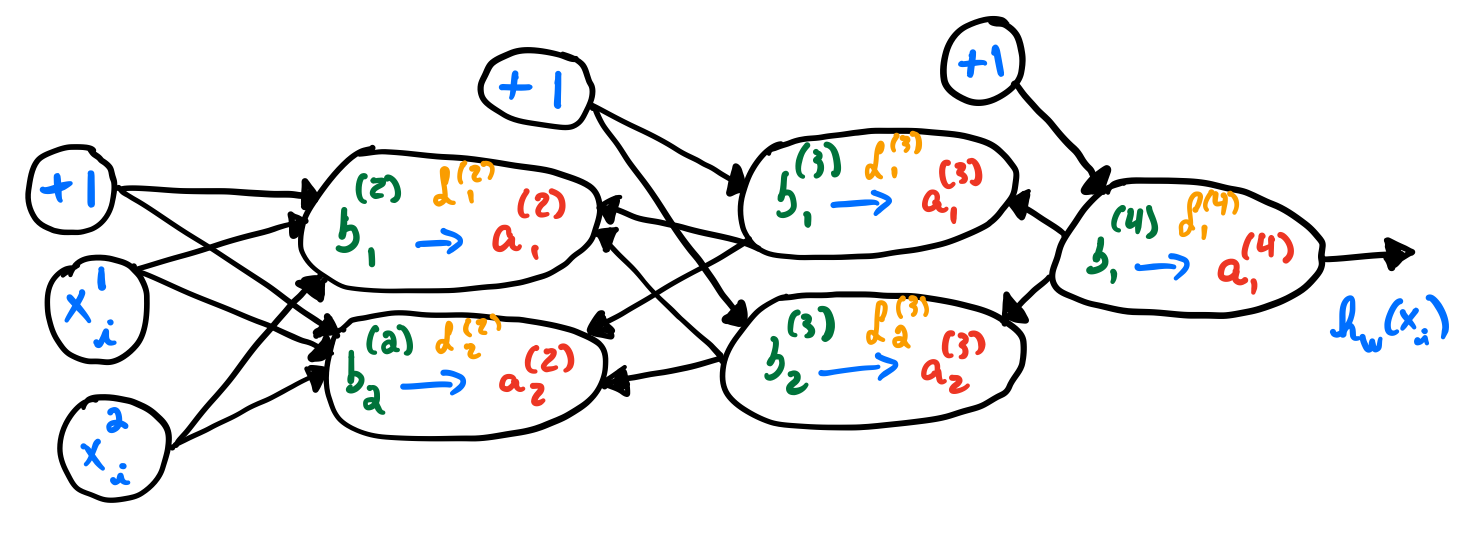
\includegraphics[scale=0.2]{./figs/Neural_Networks_Fig22.png}
\end{center}
}

\end{document}